% =====================================================================
%  Kapitel 5 – Diskussion der Ergebnisse (~3–4 Seiten)
% =====================================================================
\chapter{Diskussion der Ergebnisse}
\label{kap:diskussion}

\section{Funktionsnachweis}
\label{sec:funktionsnachweis}

\todoi{Kurz: Neffy~3.0 wurde vollständig aufgebaut und in Betrieb genommen -- was funktioniert im
Zusammenspiel (Aufwachen bei Anwesenheit, Atemerkennung, Bewegung, LEDs, Übung)? Wo wurde er
vorgeführt/getestet?}

\begin{figure}[htbp]
  \centering
  \platzhalter{Foto des fertigen Neffy~3.0}
  \caption{Neffy~3.0 im aufgebauten Zustand}
  \label{fig:neffy_fertig}
\end{figure}

\section{Messwerte und Auswertung}
\label{sec:messwerte}

\subsection{Messreihen zur Atemsensorik}
\label{sec:erg_messreihen}

Für die Atemsensorik wurden elf Messreihen in drei Gruppen aufgezeichnet: drei mit dem \ac{FSR}
(F1--F3), zwei mit Velostat und nur aufgelegten Händen (P1, P2) und sechs mit Velostat und aktivem
Mitdrücken beim Einatmen (A1--A6). Gemessen wurde mit dem in Abschnitt~\ref{sec:hw_drucksensor}
beschriebenen Aufbau am ESP32-Entwicklungsboard; beim Velostat lag ein Festwiderstand von
10\,k$\Omega$ im Spannungsteiler. Tabelle~\ref{tab:kennwerte} fasst die Kennwerte zusammen. Der
Anteil der Messwerte bei 0 bzw.\ am oberen Ende des Messbereichs (4095) zeigt, wie oft der Sensor
nur \enquote{aus} oder \enquote{voll} meldet. Der Signalhub ist die Differenz zwischen dem 95.- und dem
5.-Perzentil, solange die Hand auf dem Sensor liegt. Die Atemzüge wurden offline aus dem
geglätteten Signal bestimmt (gleitender Mittelwert über sieben Werte, Mindesthöhe eines Maximums
700 ADC-Einheiten, Mindestabstand 1{,}5\,s); daraus folgen mittlere Atemperiode und Atemfrequenz.

\begin{table}[htbp]
  \centering
  \caption{Kennwerte der Messreihen zur Atemsensorik (erzeugt aus den Rohdaten, Anhang~\ref{anh:rohdaten})}
  \label{tab:kennwerte}
  \small
  % Automatisch erzeugt von daten/tabelle_kennwerte.py -- nicht von Hand bearbeiten
\begin{tabular}{@{}l l r r r r r c r@{}}
  \toprule
  & & Dauer & \multicolumn{3}{c}{Anteil der Messwerte in \%} & Signal- & Atem- & Atem- \\
  \cmidrule(lr){4-6}
  ID & Aufbau & in s & bei 0 & bei 4095 & 100--4000 & hub & züge & frequenz \\
  & & & & & & (ADC) & & (1/min) \\
  \midrule
  F1 & \acs{FSR} & 72{,}6 & 62{,}0 & 20{,}1 & 16{,}3 & -- & -- & -- \\
  F2 & \acs{FSR} & 8{,}8 & 57{,}1 & 25{,}1 & 16{,}0 & -- & -- & -- \\
  F3 & \acs{FSR} & 18{,}9 & 63{,}9 & 0{,}0 & 36{,}1 & -- & -- & -- \\
  \addlinespace
  P1 & Velostat, aufgelegt & 32{,}2 & 6{,}2 & 1{,}4 & 82{,}9 & 455 & 0 & -- \\
  P2 & Velostat, aufgelegt & 23{,}6 & 0{,}0 & 0{,}0 & 80{,}3 & 107 & 0 & -- \\
  \addlinespace
  A1 & Velostat, aktiv & 26{,}9 & 0{,}0 & 0{,}0 & 98{,}7 & 3360 & 5 & 14{,}2 \\
  A2 & Velostat, aktiv & 51{,}0 & 8{,}0 & 0{,}0 & 89{,}8 & 3103 & 4 & 15{,}2 \\
  A3 & Velostat, aktiv & 20{,}3 & 0{,}0 & 14{,}3 & 71{,}7 & 1536 & 4 & 12{,}1 \\
  A4 & Velostat, aktiv & 25{,}4 & 0{,}0 & 14{,}0 & 82{,}6 & 1410 & 4 & 15{,}1 \\
  A5 & Velostat, aktiv & 19{,}9 & 0{,}0 & 0{,}0 & 100{,}0 & 1484 & 4 & 14{,}0 \\
  A6 & Velostat, aktiv & 28{,}2 & 0{,}0 & 3{,}7 & 95{,}6 & 2360 & 4 & 9{,}7 \\
  \bottomrule
\end{tabular}

\end{table}

\subsection{Vergleich von FSR und Velostat}
\label{sec:erg_fsr}

Die Kennwerte bestätigen die Beobachtung aus Abschnitt~\ref{sec:hw_drucksensor} quantitativ. Beim
\ac{FSR} lagen 57 bis 64\,\% aller Messwerte bei 0 und in zwei Messreihen 20 bis 25\,\% am oberen
Ende des Messbereichs; nur 16 bis 36\,\% der Werte lagen dazwischen. Der Sensor meldete damit
überwiegend nur \enquote{kein Druck} oder \enquote{voller Druck}. Beim Velostat mit aktivem
Mitdrücken lagen dagegen 72 bis 100\,\% der Werte im Zwischenbereich, sodass sich der Verlauf
eines Atemzugs abbilden lässt.

\subsection{Passive Atemerkennung}
\label{sec:erg_passiv}

Lagen die Hände nur auf dem Velostat (P1, P2), entstand ein nahezu konstantes Plateau, in dem
keine Atemzüge erkennbar waren (Abbildung~\ref{fig:passiv_aktiv}\,a). Der Signalhub betrug nur
455 bzw.\ 107 ADC-Einheiten und lag damit in derselben Größenordnung wie die Schwankungen durch
kleine, unbeabsichtigte Bewegungen der Hände. Das Gewicht der aufliegenden Hände bestimmt das
Signal; die Atembewegung verändert den Druck auf den Sensor dagegen kaum. Atmung und zufällige
Handbewegungen lassen sich so nicht zuverlässig unterscheiden. Die ursprünglich geplante passive
Erkennung ist mit diesem Aufbau daher nicht umsetzbar.

\begin{figure}[htbp]
  \centering
  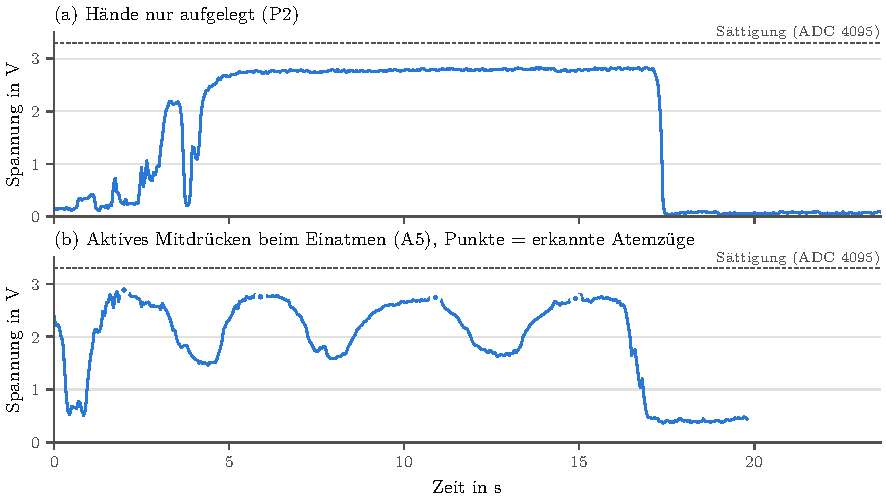
\includegraphics[width=\linewidth]{plots/velostat_aufgelegt_vs_aktiv.pdf}
  \caption{Velostat mit nur aufgelegten Händen (a, P2) und mit aktivem Mitdrücken beim
    Einatmen (b, A5); Punkte markieren die erkannten Atemzüge}
  \label{fig:passiv_aktiv}
\end{figure}

\subsection{Aktive Atemerkennung}
\label{sec:erg_aktiv}

Mit aktivem Mitdrücken zeigten alle sechs Messreihen deutliche, regelmäßige Atemzüge
(Abbildung~\ref{fig:passiv_aktiv}\,b). Der Signalhub lag mit 1410 bis 3360 ADC-Einheiten etwa
drei- bis dreißigmal so hoch wie bei nur aufgelegten Händen. In jedem Auswertefenster wurden vier
bis fünf Atemzüge erkannt; die mittlere Atemperiode lag zwischen 3{,}95 und 6{,}17\,s, was einer
Atemfrequenz von 9{,}7 bis 15{,}2 Atemzügen pro Minute entspricht. In A3 und A4 erreichten 14\,\%
der Werte das obere Ende des Messbereichs, weil zu fest gedrückt wurde; die Atemzüge blieben
trotzdem gut erkennbar. A5 lieferte die saubersten Zyklen ohne Sättigung.

Übertragen auf die Einstufung der Firmware (Abschnitt~\ref{sec:sw_atem}) entsprechen 12{,}1 bis
15{,}2 Atemzüge pro Minute 6 bis 8 Atemzügen in 30\,s und damit der Stufe \enquote{normal}; die
langsamste Messreihe A6 mit 9{,}7 pro Minute läge mit knapp 5 Atemzügen in 30\,s bei
\enquote{entspannt}. Die Ergebnisse sind plausibel, unterliegen aber zwei Einschränkungen: Die
Messungen fanden am Entwicklungsboard und nicht im fertigen Sensoreinsatz statt, und die
Atemzüge wurden offline bestimmt, nicht mit der Erkennung der Firmware.
\todo{Gibt es Tests der Atemerkennung am fertigen Neffy (Erkennungsrate, Einstufung)?}

\subsection{Anwesenheitserkennung}
\label{sec:erg_anwesenheit}

\todoi{Ergebnisse: Ab welcher Entfernung wird eine Person erkannt, wie schnell, Reaktion beim
Vorbeigehen, Fehlauslösungen? Laut Abstimmungsaufnahme der Firmware: direkt davor $+4$ bis
$+6$\,K, in 1\,m etwa $+2$\,K über Raumtemperatur. Messdaten/Logs vorhanden
(\texttt{logs/thermal-*.csv})?}

\section{Evaluation gegen die Anforderungen}
\label{sec:evaluation}

Tabelle~\ref{tab:evaluation} bewertet die Anforderungen aus Tabelle~\ref{tab:anforderungen}.

\begin{table}[htbp]
  \centering
  \caption{Erfüllungsgrad der Anforderungen (\checkmark\ erfüllt, $\circ$ teilweise, -- nicht erfüllt)}
  \label{tab:evaluation}
  \small
  \begin{tabular}{@{}l >{\raggedright\arraybackslash}p{3.6cm}
                    >{\centering\arraybackslash}p{1.3cm}
                    >{\raggedright\arraybackslash}p{6.6cm}@{}}
    \toprule
    Nr. & Anforderung & Status & Begründung \\
    \midrule
    A1 & Anwesenheit erkennen & \todoi{?} & \todoi{Begründung} \\
    A2 & Reaktion auf Anwesenheit & \todoi{?} & \todoi{Begründung} \\
    A3 & Einatemzüge erkennen, Atemfrequenz bestimmen & $\circ$
       & Im Labortest klar erkennbar (9{,}7--15{,}2/min); am fertigen Roboter nicht gemessen
         \todoi{bestätigen} \\
    A4 & Einstufung an den Raspberry Pi & \todoi{?} & \todoi{Begründung} \\
    A5 & Hub mit beiden Händen & \todoi{?} & \todoi{Begründung} \\
    A6 & Gestaltung nach Zielbild & \checkmark
       & Runde, weniger kantige Form mit Taschen umgesetzt \\
    A7 & Hände sicher in Taschen & $\circ$
       & Hände liegen gesichert; Position von Händen und Ellbogen etwas zu hoch \\
    A8 & Zugang zur Elektronik & \checkmark
       & Oberkörper magnetisch, ohne Werkzeug abnehmbar; Unterkörper mit sechs Schrauben \\
    A9 & Druck auf vorhandenen Druckern & \checkmark
       & Alle Teile gedruckt; dafür Teilung in 16 Druckteile nötig \\
    \bottomrule
  \end{tabular}
\end{table}

\section{Schwachstellen}
\label{sec:schwachstellen}

\begin{itemize}
  \item \textbf{Keine passive Atemerkennung:} Das ursprüngliche Ziel, die Atmung allein über die
        aufgelegten Hände zu erkennen, wurde nicht erreicht (Abschnitt~\ref{sec:erg_passiv}). Die
        aktive Erfassung erfordert, dass die Nutzer:innen bewusst mitdrücken.
  \item \textbf{Sättigung bei festem Druck:} Wird zu fest gedrückt, erreicht das Signal das obere
        Ende des Messbereichs (A3, A4). Die Erkennung bleibt möglich, die Signalform geht aber
        verloren.
  \item \textbf{Ergonomie:} Durch die Größe von Neffy~3.0 liegen Hände und Ellbogen etwas zu hoch;
        dieser Punkt wurde im Entwurf zu wenig beachtet. Als einfache Abhilfe dienen kleine Kissen
        links und rechts unter den Ellbogen.
  \item \textbf{Schrittmotoren und Referenzfahrt:} \todoi{Probleme konkret: z.\,B. verlorene
        Schritte, wenn eine Achse beim Start auf dem Endschalter stand; Endlosschleife bei der
        Referenzfahrt des Kopfes (in der Firmware behoben) -- weitere?}
  \item \textbf{Zweckentfremdeter Befehl:} Der Befehl \texttt{DISABLE\_MOTORS} schaltet die Motoren
        nicht ab, sondern dient als Startsignal einer Übung. Der Name passt nicht zur Bedeutung und
        erschwert die Wartung der Schnittstelle.
  \item \textbf{Fertigung:} Es gibt nur eine Gehäuseversion; Toleranzen wurden nicht vorab an
        Testkörpern bestimmt, sodass häufig nachgebohrt werden musste. Die Klebestellen erforderten
        viel Nachbearbeitung.
  \item \textbf{Keine Nutzerstudie:} Anders als zu Neffy~1.0 und 2.0 gibt es zu Neffy~3.0 noch keine
        Evaluation mit Nutzer:innen.
\end{itemize}

\section{Eigene Ideen}
\label{sec:eigene_ideen}

\todoi{Bestätigen bzw.\ ergänzen -- Vorschlag: Übernahme und Umsetzung des gesamten Gehäuses aus
eigener Initiative; modularer Aufbau mit Magneten; Wechsel von passiver zu aktiver Atemerfassung
über die Taschen (zugleich Touch-Eingabe); Sensoreinsatz zum Einstecken; selbstkalibrierende
Klick- und Druckerkennung; lernende Raumtemperatur bei der Anwesenheitserkennung;
LED-Rückmeldung beim Atmen. Wer was (Badre/Younes): ganz am Ende.}
